
\documentclass[tikz,border=8pt]{standalone}
\usepackage{amsmath}
\begin{document}
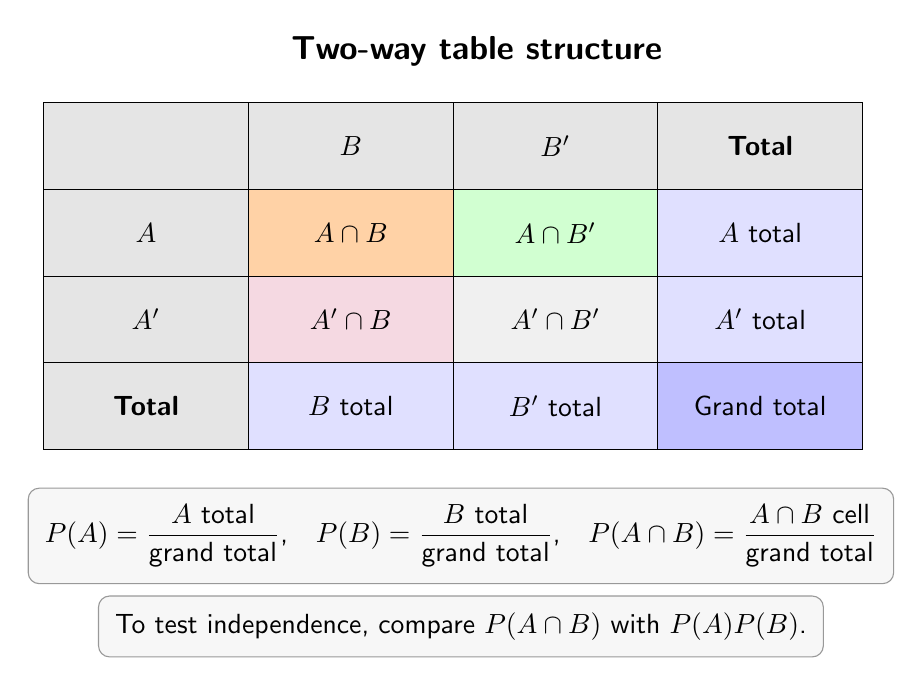
\begin{tikzpicture}[font=\sffamily,cell/.style={draw=black, minimum width=2.6cm, minimum height=1.1cm, align=center},head/.style={cell, fill=black!10, font=\sffamily\bfseries},focus/.style={cell, fill=orange!35},total/.style={cell, fill=blue!12},note/.style={draw=black!40, rounded corners, fill=black!3, align=center, inner sep=6pt}]
\node[font=\sffamily\bfseries\large] at (4.2,1.2) {Two-way table structure};
\node[head] at (0,0) {};\node[head] at (2.6,0) {$B$};\node[head] at (5.2,0) {$B'$};\node[head] at (7.8,0) {Total};
\node[head] at (0,-1.1) {$A$};\node[focus] at (2.6,-1.1) {$A\cap B$};\node[cell, fill=green!18] at (5.2,-1.1) {$A\cap B'$};\node[total] at (7.8,-1.1) {$A$ total};
\node[head] at (0,-2.2) {$A'$};\node[cell, fill=purple!15] at (2.6,-2.2) {$A'\cap B$};\node[cell, fill=gray!12] at (5.2,-2.2) {$A'\cap B'$};\node[total] at (7.8,-2.2) {$A'$ total};
\node[head] at (0,-3.3) {Total};\node[total] at (2.6,-3.3) {$B$ total};\node[total] at (5.2,-3.3) {$B'$ total};\node[total, fill=blue!25] at (7.8,-3.3) {Grand total};
\node[note] at (4.0,-4.95) {$P(A)=\dfrac{A\text{ total}}{\text{grand total}}$,\quad $P(B)=\dfrac{B\text{ total}}{\text{grand total}}$,\quad $P(A\cap B)=\dfrac{A\cap B\text{ cell}}{\text{grand total}}$};
\node[note] at (4.0,-6.1) {To test independence, compare $P(A\cap B)$ with $P(A)P(B)$.};
\end{tikzpicture}
\end{document}
